\documentclass[11pt]{article}
\usepackage[utf8]{inputenc}
\usepackage{geometry}
\usepackage{booktabs}
\usepackage{graphicx}
\usepackage{hyperref}
\usepackage{amsmath}
\usepackage{amssymb}
\usepackage{caption}

\title{Preferences in AI Project Report}
\author{Pratik Deshmukh}
\date{\today}

\begin{document}

\maketitle

\section{Introduction}
This report presents experiments on free-riding in sequential decision-making
under different \emph{statistical cultures}, following the framework of
\cite{lackner2023freeriding}. Our goal is to replicate the structure of Section~5
of that work while extending it with additional statistical cultures and updated
parameter settings.

\section{Background}

\subsection{Multi-Issue Model}
We study sequential decision-making in \emph{multi-issue elections}, where a set
of voters must decide on several issues, each with multiple candidates. Each
voter submits approval preferences for all candidates on each issue. A voting
rule is then applied issue by issue to determine the collective outcome.

\subsection{Voting Rules}
We focus on two major families of rules, following \cite{lackner2023freeriding}:

\begin{itemize}
    \item \textbf{Sequential Utilitarian Rule:} selects in each issue the
    candidate with the highest total number of approvals. This rule is
    equivalent to the mean OWA and is known to be immune to manipulation.
    \item \textbf{Thiele-Based Rules:} a general class where voter satisfaction
    decreases marginally as more of their approved candidates are selected.
    We evaluate sequential Thiele rules with parameters $x \in \{1,5,7\}$,
    where $x=0$ corresponds to utilitarian aggregation.
    \item \textbf{OWA-Based Rules:} aggregate voter satisfaction using Ordered
    Weighted Averages (OWAs). Following \cite{lackner2023freeriding}, we use
    normalized positive weights (no zeros) interpolating between utilitarian
    and leximin behavior. We evaluate parametric OWA rules with
    $x \in \{1,5,10,15\}$, and include the explicit
    \emph{leximin OWA} as the limiting case.
\end{itemize}

\subsection{Statistical Cultures}
The way preferences are generated strongly influences manipulation risks.
We consider four cultures:
\begin{itemize}
    \item \textbf{p-IC}: per-issue impartial culture, sampling approvals
    independently with probability $p=0.5$.
    \item \textbf{Disjoint Groups}: voters are divided into $g=2$ groups with
    internally aligned preferences.
    \item \textbf{Resampling Model}: preferences are generated by resampling
    with parameters $(p, \phi) = (0.5, 0.5)$ controlling randomness and correlation.
    \item \textbf{Hamming Noise}: preferences are first generated from another
    culture and then perturbed by flipping approvals with small probability
    $\epsilon=0.1$ per issue. This noise model captures robustness under
    small random perturbations.
\end{itemize}

\subsection{Risk Metrics}
We evaluate manipulation opportunities using the following metrics:
\begin{itemize}
    \item \textbf{Trials:} total number of manipulation attempts.
    \item \textbf{Successes:} number of manipulations that improved the manipulator’s outcome.
    \item \textbf{Harms:} number of manipulations that backfired on the manipulator.
    \item \textbf{Success rate:} proportion of trials with a successful manipulation.
    \item \textbf{Harm rate:} proportion of trials with a harmful manipulation.
    \item \textbf{Risk:} ratio of harms to successes (conditional probability of harmful manipulation).
\end{itemize}

\section{Methodology}
We replicate the experiments from Section~5 of \cite{lackner2023freeriding},
using four statistical cultures: impartial culture (p-IC), disjoint groups,
the $(p, \phi)$-resampling model, and the Hamming-noise model. For each culture,
we run multiple random seeds and compare risk metrics under sequential
utilitarian, sequential Thiele rules ($x=1,5,7$), and OWA rules ($x=1,5,10,15$, plus leximin).

\subsection{Parameters}
The main parameters used in our experiments are:

\begin{itemize}
    \item Number of voters: $n=20$
    \item Number of issues: $k=5$
    \item Candidates per issue: $c=4$
    \item Random seeds: $200$
    \item Cultures and hyperparameters: as defined in the previous subsection.
\end{itemize}

All configurations were executed using our unified experimental pipeline,
which produces both tabular summaries and risk plots.

\section{Results}
The combined results table is automatically generated by the experiment
pipeline. The table below is included directly from the output file:

\begin{table}[h!]
\centering
\resizebox{\textwidth}{!}{%
\input{tables/combined.tex}
}
\caption{Combined results across cultures and rules. Risk metrics include trials,
successes, harms, success and harm rates, and risk (harms/successes).}
\label{tab:combined}
\end{table}

\subsection{Per-Culture Comparisons}
To visualize the trends, we show manipulation risks by rule family (Thiele and OWA)
for each statistical culture.

\paragraph{p-IC.}
\begin{figure}[h!]
\centering
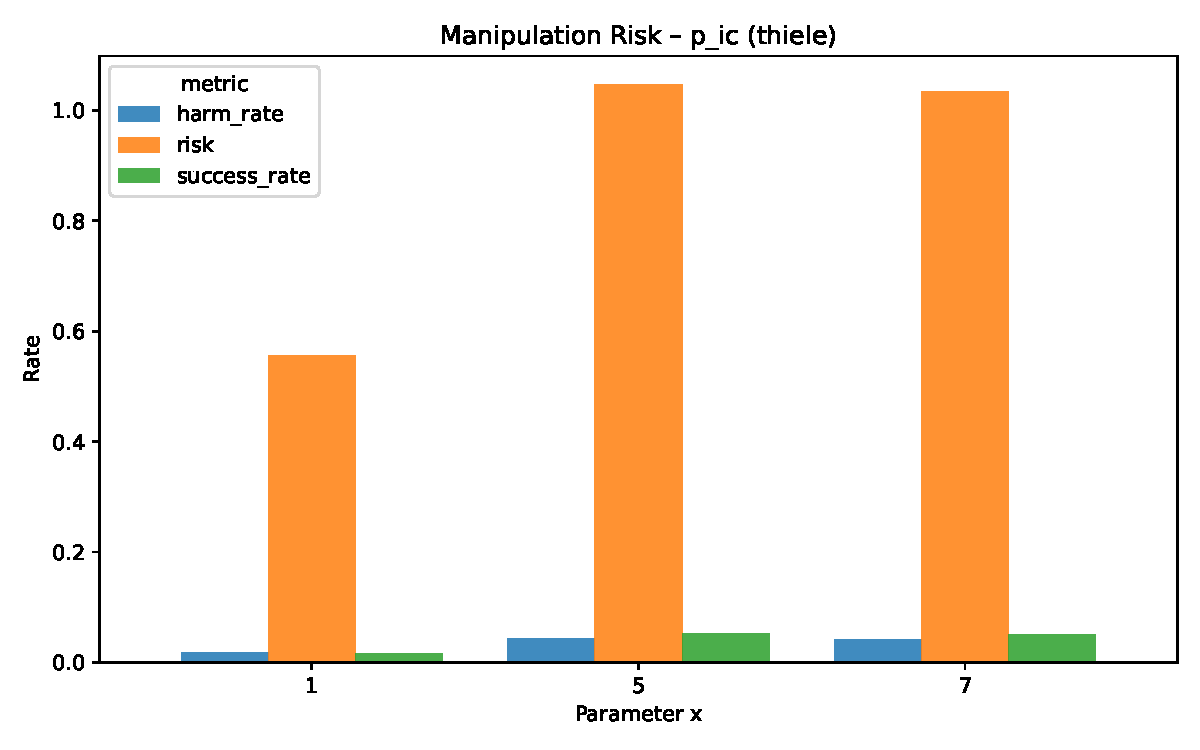
\includegraphics[width=0.7\textwidth]{figures/risk_p_ic_thiele.pdf}
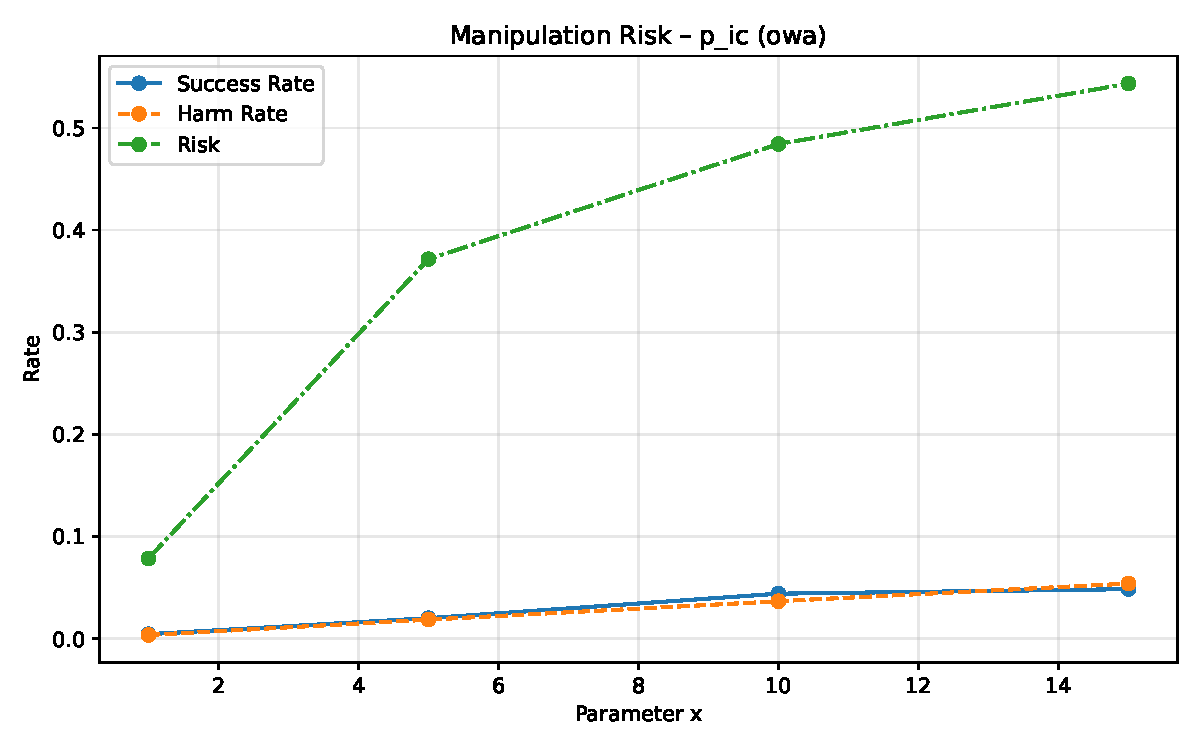
\includegraphics[width=0.7\textwidth]{figures/risk_p_ic_owa.pdf}
\caption{Manipulation risk under p-IC culture. Top: Thiele rules. Bottom: OWA rules.}
\end{figure}
Under p-IC, both Thiele and OWA families show mild manipulation rates.
OWA rules exhibit slightly lower success and harm rates, while leximin remains
largely immune. This matches the expected robustness of random independent
preferences.

\paragraph{Disjoint Groups.}
\begin{figure}[h!]
\centering
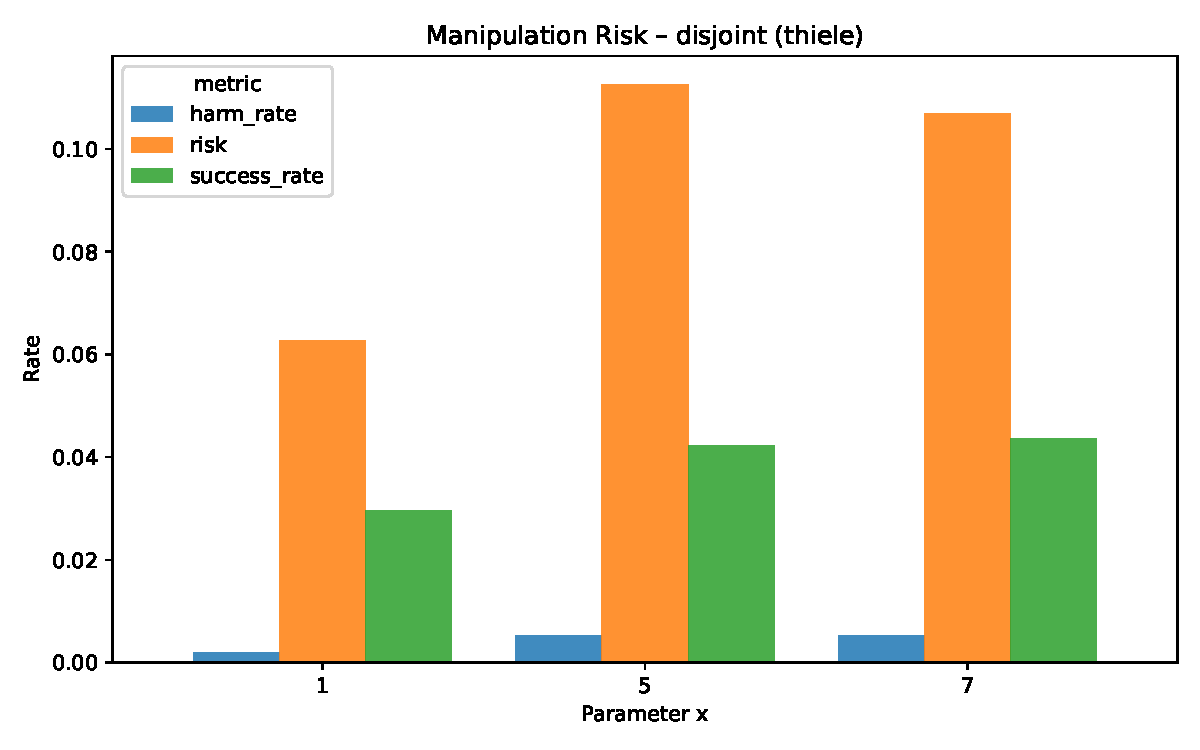
\includegraphics[width=0.7\textwidth]{figures/risk_disjoint_thiele.pdf}
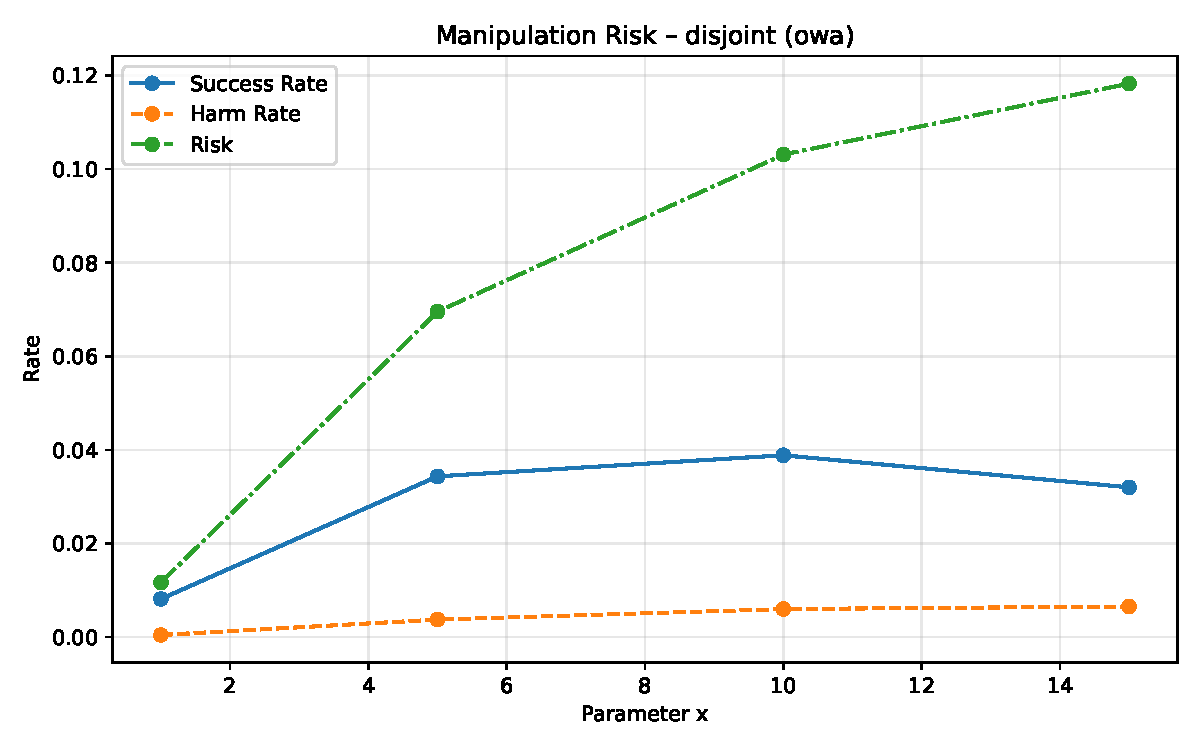
\includegraphics[width=0.7\textwidth]{figures/risk_disjoint_owa.pdf}
\caption{Manipulation risk under disjoint-group culture. Top: Thiele rules. Bottom: OWA rules.}
\end{figure}
Disjoint group structures introduce correlated preferences. Manipulation success
increases slightly for Thiele rules, but harm rates stay very low, indicating that
free-riding is relatively safe when preferences are clustered.

\paragraph{Resampling Model.}
\begin{figure}[h!]
\centering
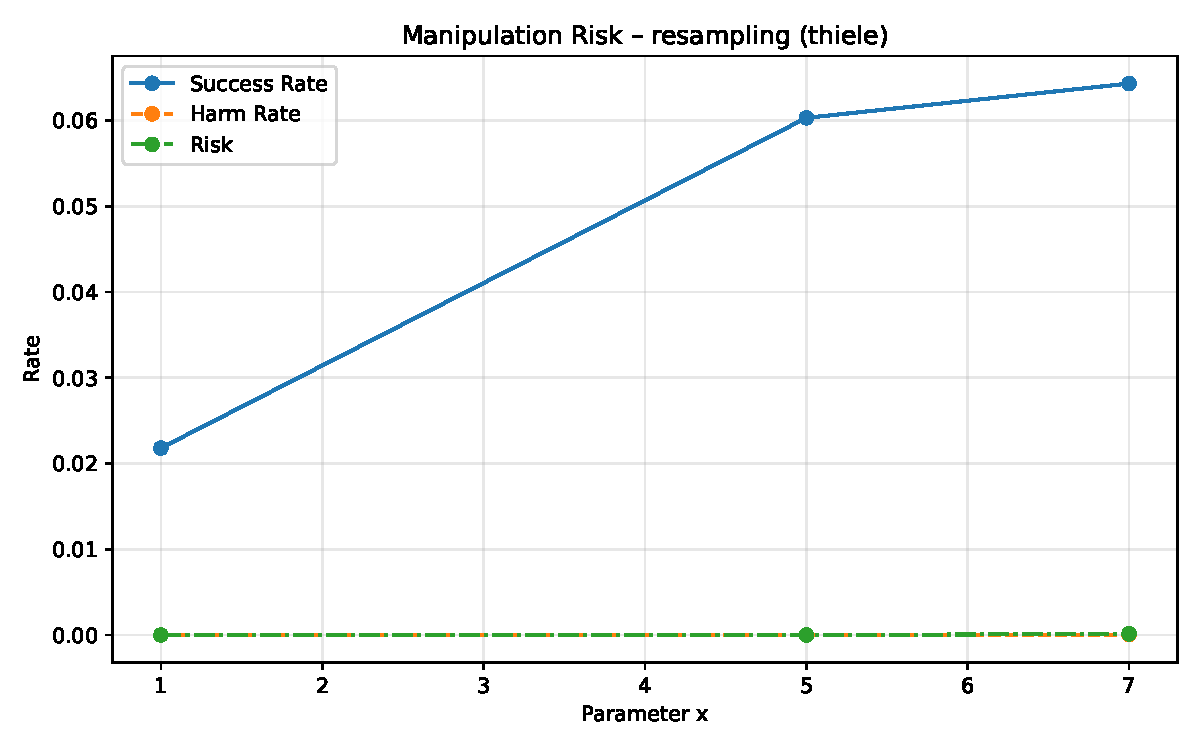
\includegraphics[width=0.7\textwidth]{figures/risk_resampling_thiele.pdf}
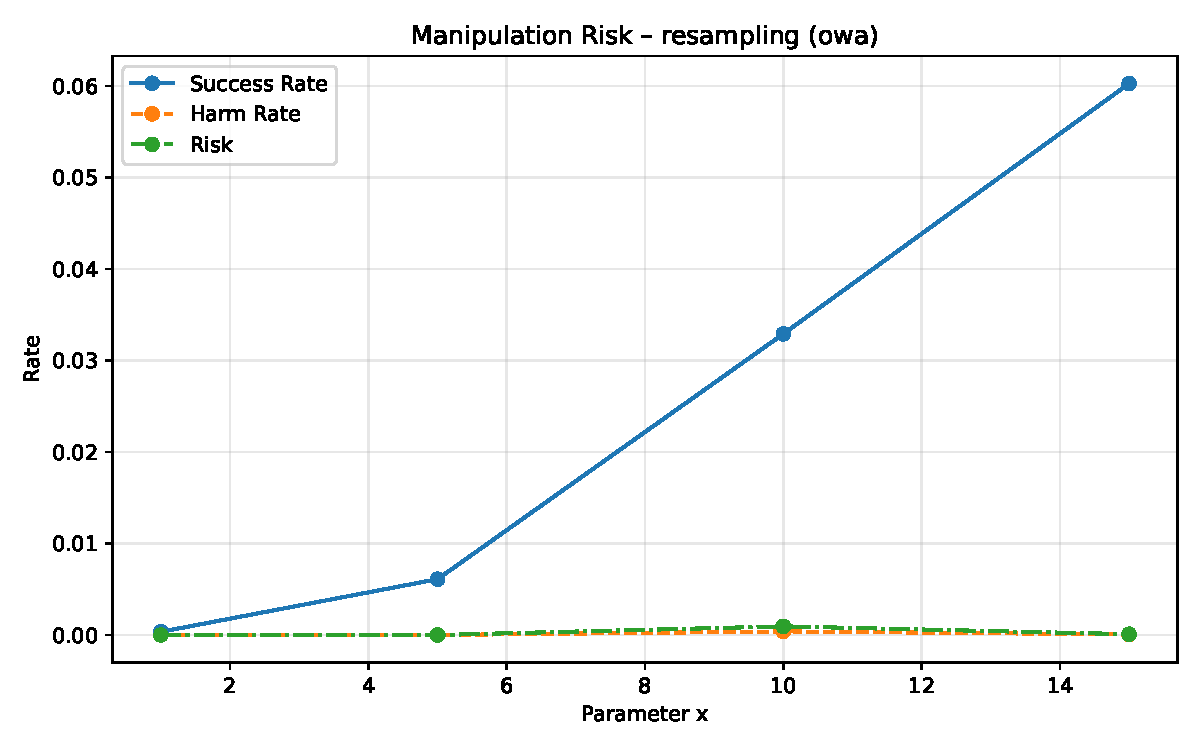
\includegraphics[width=0.7\textwidth]{figures/risk_resampling_owa.pdf}
\caption{Manipulation risk under resampling culture. Top: Thiele rules. Bottom: OWA rules.}
\end{figure}
The resampling culture yields intermediate results between p-IC and disjoint.
Thiele and OWA rules exhibit low but nonzero manipulation potential. Higher $x$
values slightly increase risk, consistent with greater proportionality.

\paragraph{Hamming Noise.}
\begin{figure}[h!]
\centering
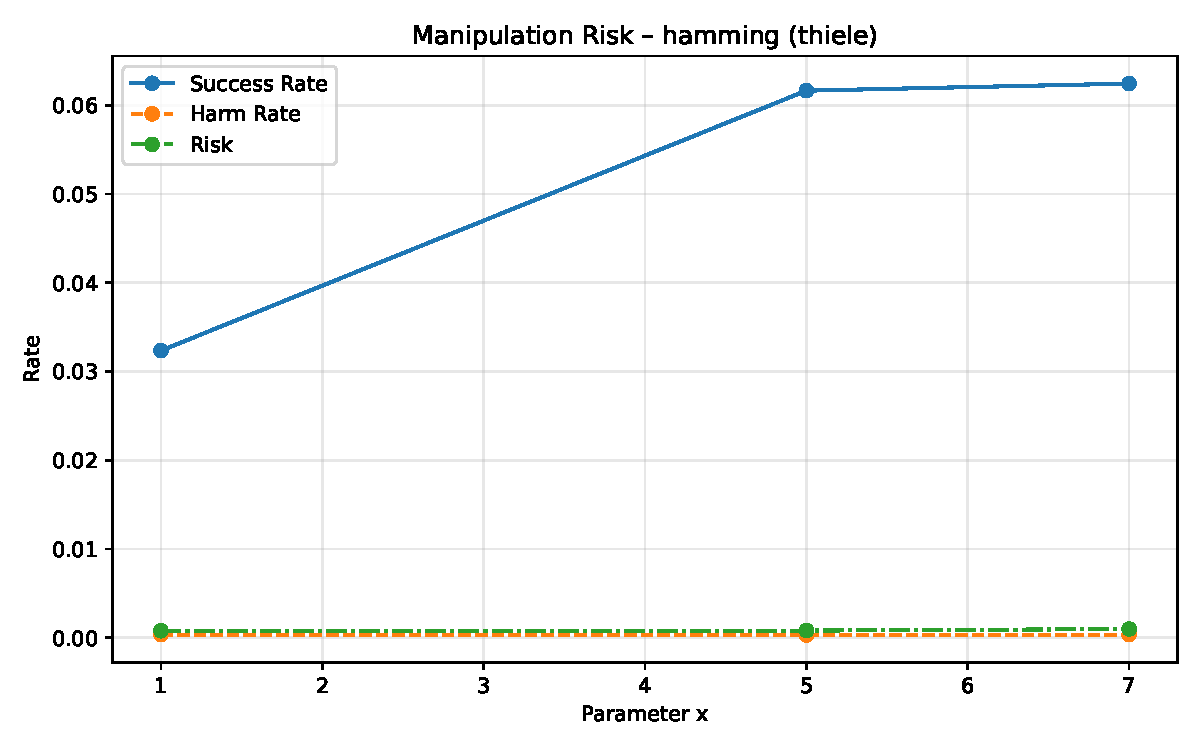
\includegraphics[width=0.7\textwidth]{figures/risk_hamming_thiele.pdf}
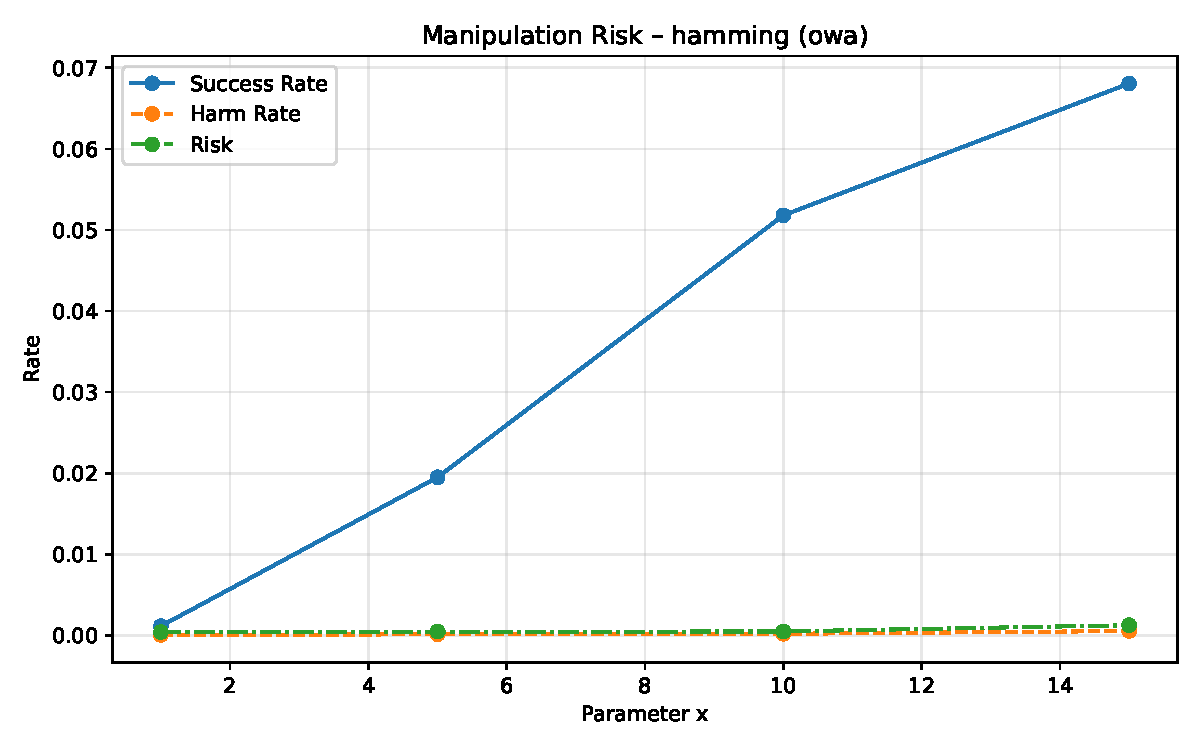
\includegraphics[width=0.7\textwidth]{figures/risk_hamming_owa.pdf}
\caption{Manipulation risk under Hamming-noise culture. Top: Thiele rules. Bottom: OWA rules.}
\end{figure}
Hamming perturbations add random noise to structured preferences. As expected,
this causes mild increases in both success and harm rates. Leximin remains
mostly stable, confirming its resilience to random perturbations.

\section{Discussion}
Our experiments highlight the dependence of manipulation risk on both the
voting rule and the statistical culture.

\paragraph{Effect of Statistical Cultures.}
The \emph{p-IC} culture exhibits moderate manipulation opportunities.
The \emph{disjoint} model produces clearer group structures, increasing the
chance that one group can manipulate effectively. The \emph{resampling} model
shows behavior similar to p-IC but slightly more correlated outcomes, while
\emph{Hamming noise} introduces random fluctuations that may both increase or
reduce risks depending on the rule.

\paragraph{Effect of Voting Rules.}
The \emph{utilitarian rule} (equivalently mean OWA) is immune to manipulation.
Thiele rules with larger $x$ increase proportionality but also marginally
increase free-riding potential. OWA rules interpolate between utilitarian and
leximin: intermediate parameters show moderate manipulation risks, while the
\emph{leximin rule} remains the most resistant to manipulation, in line with
our results (very low success and harm rates).

\paragraph{Risk Metrics.}
Across all settings, harm rates remain small but nonzero, confirming that
attempts at manipulation carry measurable risks. The ratio of harms to
successes (\emph{risk}) stays well below 1, indicating that manipulators more
often succeed than fail—but not without potential downsides.

\section{Conclusion}
Our experiments confirm that the choice of statistical culture strongly
influences manipulation risks. Cultures with correlated preferences (e.g.,
disjoint, resampling) can increase opportunities for manipulation, while random
noise can unpredictably alter them.

Across voting rules, utilitarian aggregation is immune. Thiele and OWA rules
illustrate clear trade-offs: increasing fairness or proportionality often
slightly increases manipulation risk, but leximin consistently shows the
highest robustness. These findings align closely with the theoretical and
empirical trends observed by \cite{lackner2023freeriding}.

Future work could extend these experiments by exploring richer parameter grids
for $(p,\phi)$ and $\epsilon$, as well as scaling to larger electorates or
mixed-issue dependencies. Replicating the visualization style of
\cite{lackner2023freeriding} for welfare and risk together would further
improve interpretability.

\section*{Repository}
The full project code and report sources are available at: \\
\href{https://github.com/inquisitour/preferences-in-ai}{github.com/inquisitour/preferences-in-ai}

\bibliographystyle{plain}
\bibliography{references}

\end{document}
% !TEX root = report.tex
